%%%%%%%%%%%%%%%%%%%%%%%%%%%%%%%%%%%%%%%%%%%%%%%%%%%%%%%%%%%%%%%%%%%%%%%%%%%%%%%%
%2345678901234567890123456789012345678901234567890123456789012345678901234567890
%        1         2         3         4         5         6         7         8

\documentclass[letterpaper, 10 pt, conference]{ieeeconf}  % Comment this line out if you need a4paper

%\documentclass[a4paper, 10pt, conference]{ieeeconf}      % Use this line for a4 paper

\IEEEoverridecommandlockouts                              % This command is only needed if 
                                                          % you want to use the \thanks command

\overrideIEEEmargins                                      

% Needed to meet printer requirements.

% See the \addtolength command later in the file to balance the column lengths
% on the last page of the document

% The following packages can be found on http:\\www.ctan.org
%\usepackage{graphics} % for pdf, bitmapped graphics files
%\usepackage{epsfig} % for postscript graphics files
%\usepackage{mathptmx} % assumes new font selection scheme installed
%\usepackage{times} % assumes new font selection scheme installed
%\usepackage{amsmath} % assumes amsmath package installed
%\usepackage{amssymb}  % assumes amsmath package installed


%\title{\LARGE \bf Fast Run-time Verified Reachability for Safe Autonomous Operations} 
\title{\LARGE \bf A Framework for Verified Fast Run-time Reachability for Safe Autonomous Systems Operations} 

\newcommand{\subparagraph}{}
\newcommand\NB[1]{$\spadesuit$\footnote{NB: #1}}
\newcommand\EY[1]{$\clubsuit$\footnote{EY: #1}}

\renewcommand{\Re}{\mathbb{R}}
\newcommand{\Ze}{\mathbb {Z}}
\newcommand{\De}{\mathbb {D}}
\newcommand{\Pe}{\mathbb {P}}
\newcommand{\Ne}{\mathbb {N}}

\usepackage{graphicx}
\usepackage{epstopdf}
\usepackage{amsmath}
\usepackage{amssymb}
\usepackage{subfigure}
\usepackage{multirow}
\usepackage{pbox}
\usepackage{algorithm}
\usepackage{algpseudocode}
\usepackage{titlesec}
\usepackage{bm}
\usepackage{url}
\usepackage{dblfloatfix} 

\newtheorem{problem}{Problem}
\newtheorem{lemma}{Lemma}

\renewcommand{\baselinestretch}{0.95}

\begin{document}

\maketitle
\thispagestyle{empty}
\pagestyle{empty}
%!TEX root = IROS2019_DNN.tex

\begin{abstract}

\end{abstract}
%!TEX root = IROS2019_DNN.tex

\begin{section}{Introduction} \label{sec:intro}

Autonomous vehicles are becoming increasingly popular and part of our daily lives. Autonomous transportation, package and food delivery, firefighting, law-enforcement, medical service, hobby, and house-hold applications are just some examples where the use of robotics is advantageous over other technologies. 

As they find their way into our society it becomes critical during run-time to guarantee safety against unpredictable uncertainties and disturbances. In fact, while model-driven motion planning and control techniques can be robust against noises and disturbances, they cannot prevent deviations from the desired behavior during the system operation which could potentially lead to unsafe states (e.g. crashing into an obstacle in the environment due to excessive wind disturbance). In order to assure safety of the autonomous operations, it is necessary to take the effect of noises and disturbances into consideration during planning. Traditional reachability analysis tools like \NB{CITE} have demonstrated to be very effective in predicting future states of the system by utilizing the knowledge about the system model and dynamics. However they are computationally expensive making them hard to use as run-time monitors, subject of this paper.

On the other hand machine learning provides a potentially innovative way to enable fast reachability analysis. Unfortunately, the lack of understanding of how machine learning works, makes it challenging to provide guarantees for autonomous systems in safety-critical operations.

To deal with these challenges, in this work we present a novel verified learning-enabled framework for fast run-time monitoring of autonomous systems. In our scheme, presented in Fig. ~\ref{fig:gen_app}  a verified deep neural network (DNN) is trained to recognize safe and unsafe trajectories for a quadrotor UAV in a obstacle populated environment. Training is performed by considering a library of trajectories and their associated reachable sets. A trajectory is labeled safe if its reachable tube doesn't collide with any obstacle while it is marked unsafe otherwise. Differently from most of the work in the literature, here we verify the validity of our trained DNN by using our recent tool VERISIG \cite{IvanovVerisig18} in which \NB{brief explanation about the tool}. 

At runtime, the verified and trained DNN is used to decide about the safety of a trajectory from an untrained initial state under the effect of noise and disturbance.
%will then decide if a new trajectory is safe or not under the effect of noise and disturbance. 
If unsafe, a new trajectory is computed by increasing the distance to keep from the obstacles in the environment and testing again for safety. 

%In the event that a trajectory is found unsafe, a new trajectory is computed by increasing the distance to keep from the obstacles in the environment and test

%Over the recent years, the autonomous vehicles have started to become a part of our daily lives. Package delivery robots, autonomous cars, hobby and service robots are just a few example of commonly used autonomous systems. As they become more commonplace, assuring the safety of autonomous operations gains even more importance.
%
%Even with the advanced control and planning algorithms, an autonomous system may reach unsafe states due to  uncertainties in real world such as disturbances, measurement and input noises. In order to assure the safety of the autonomous operations under these conditions, it is necessary to take the effect of noises and disturbances into consideration during planning. Traditional reachability tools are widely used to predict the future states of a hybrid system by utilizing the knowledge about system model and dynamics. Although they are powerful tools for assessing the safety of an autonomous system, they suffer from the curse of dimensionality. For hybrid systems with large state space, it becomes very challenging to analyze their reachability with traditional tools. 

%In this work, for assuring safety in autonomous operations at run-time, we introduce a verified machine learning based framework as presented in Fig.~\ref{fig:gen_app}. 
%At offline stage, various trajectories from different initial positions in the environment to a goal position are generated and the desired distance to keep from the obstacles (avoid distance) is specified by the user. The initial positions-avoid distance pairs are labeled as safe or unsafe based on the intersection of reachable sets with the obstacles in the environment. As a reachability tool, we use a simulation-based approach using the worst case scenario assumptions, but it should be noted that the general framework is independent of the choose of reachability tool. The set of safety labeled initial positions are then used to train a deep neural network (DNN) and the network is verified using the verification tool called Verisig \cite{IvanovVerisig18}. At the online stage, the verified and trained network is used in order to make decisions about the safety of a trajectory from an untrained initial position. If the planned trajectory is predicted to be safe, the plant can execute the trajectory, otherwise replanning is required.

\NB{the contribution needs to be fixed...I'll take care of this}The contribution of the proposed framework is twofold: 1) we assure the safety of an autonomous system regardless of the planning algorithm, 2) a verified safety decision is made fast at run-time. The proposed approach makes it possible to eliminate the need for the traditional and computational expensive reachability tools, as the proposed approach makes the same predictions as such tools would make in a much faster way.

The rest of the paper is organized as follows: In Section~\ref{sec:rel_lit} we give a review of related literature. We provide details about the system and controller models in Section~\ref{sec:model}, and we explain the proposed approach in details in Section~\ref{sec:method}. The proposed approach is validated with simulations and experiments in Sections~\ref{sec:simulation} and \ref{sec:experiment} respectively. Finally we draw conclusions and discuss about future work in Section~\ref{sec:conclusion}.

\begin{figure}[t]
	\centering
	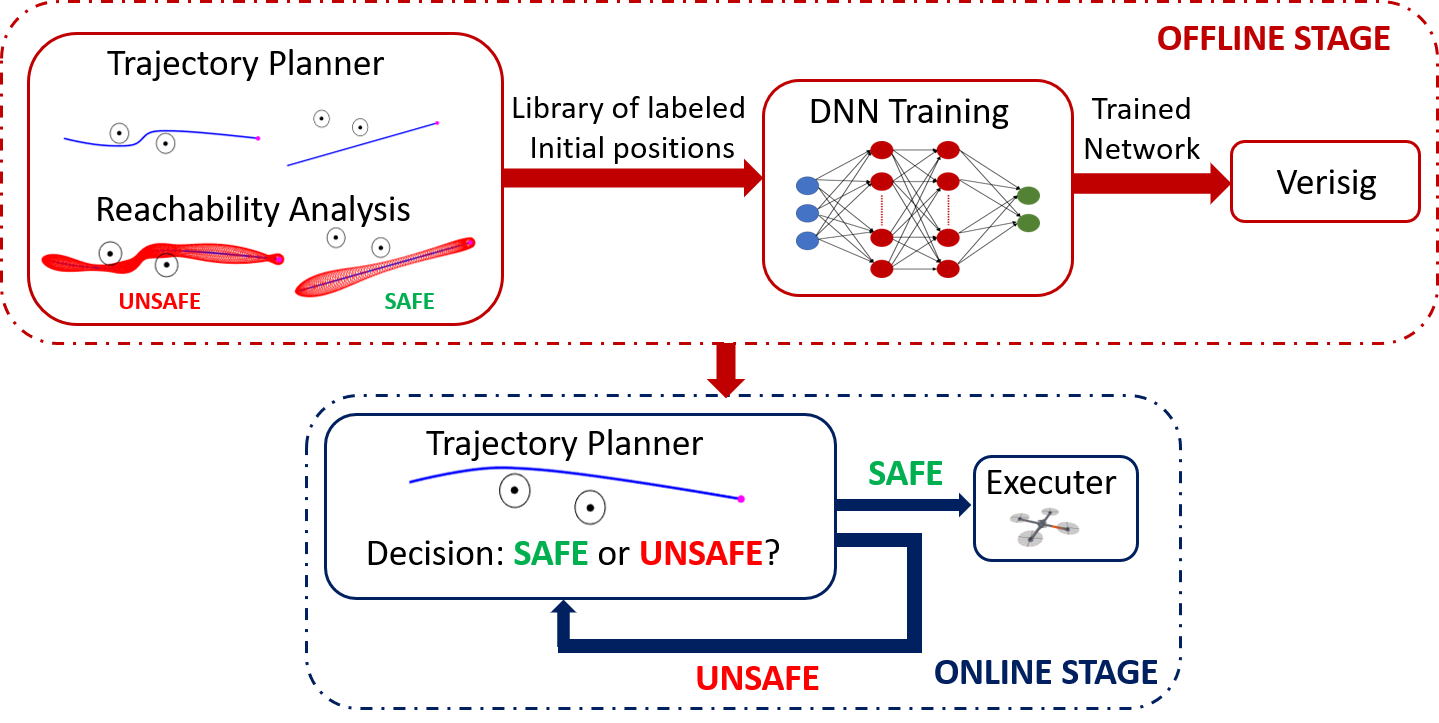
\includegraphics[width=0.45\textwidth]{figures/general_approach}
	\caption{General approach.} 
	\label{fig:gen_app}
\end{figure}
\NB{we need to change this figure. I don't like executer...let's use controller and plant instead}
\end{section}


%!TEX root = IROS2019_DNN.tex

\begin{section}{Related Work} \label{sec:rel_lit}
\EY{Related literature part will include the work with classical reachability analysis, DNNs and verification tools.}
\end{section}
%!TEX root = IROS2019_DNN.tex
	
\begin{section}{Problem Formulation} \label{sec:problem}
	In this work we are interested in predicting if a system will be able to safely reach its goal state from a given initial state. Formally this problem can be casted as follows:
	
	\textbf{Problem 1: \textit{Run-time Safety Assurance}:}
	Given the initial state of the system $ \boldsymbol{x}_0 $, at run time, predict whether the system is able to safely follow an obstacle free trajectory to a final goal under bounded disturbance, and measurement and process noises. Safety is satisfied if the following condition holds:
%	The system is safe if the following safety condition is satisfied:
	\begin{itemize}
		\item{Safety Constraint:}	
		\[ | \boldsymbol{p}(t) -\boldsymbol{p}_{o,i} | \geq r_{o,i}, \hspace{5pt} \forall t \in [0,T], \hspace{5pt} \forall i \in [0,n_o] \]	
	\end{itemize}
	where $ \boldsymbol{p}(t) $ is the position of the vehicle, $ \boldsymbol{p}_{o,i} $ and $ r_{o,i} $ are the position and the distance from the $ i^{\text{th}} $ obstacle respectively, $ n_o $ is the number of obstacles in the environment, and $ T $ is the duration of the operation. It is assumed that the obstacles are static with known positions and the system dynamics are invriants.
	\end{section}
	For ease of discussion in this work we consider that the goal position is unchanged and the disturbance is unknown but not changing during the interval of time in which it is active through the mission of the system. 

% !TEX root = IROS2019_DNN.tex

\begin{section}{System Models} \label{sec:model}
In this section we are going to explain the dynamic model of a quadrotor UAV and the controller model; then we are going to define the overall system as a hybrid system.

\subsection{Quadrotor UAV Dynamical Model}
A quadrotor can be modeled using the following $12^\text{{th}}$ order state vector:
\begin{equation*}
\bm{x} = \begin{bmatrix}\bm{p}_q^{\mathsf{T}} & \phi & \theta & \psi & v_x & v_y & v_z & \omega_{x} & \omega_{y} & \omega_{z}\end{bmatrix}^{\mathsf{T}}
\end{equation*}
where $\bm{p}_q=[x \; y \; z]^{\mathsf{T}}$ is the world frame position, $v_{x}$, $v_{y}$ and $v_z$ are the world frame velocities, $\phi$, $\theta$ and $\psi$ are the roll, pitch and yaw Euler angles and $\omega_{x}$, $\omega_{y}$ and $\omega_{z}$ are the body frame angular velocities \cite{BezzoAHS17, BezzoIROS2016}. The quadrotor has nonlinear dynamics: $ \dot{\boldsymbol{x}} = f(\boldsymbol{x}, \boldsymbol{u}, \boldsymbol{d}) $ where $ \boldsymbol{u} =  \begin{bmatrix} u_1 & u_2 & u_3 & u_4 \end{bmatrix} = \begin{bmatrix} F & M_1 & M_2 & M_3 \end{bmatrix} $ is the thrust and moment inputs, and $ \boldsymbol{d} = \begin{bmatrix} d_x & d_y & d_z \end{bmatrix} $ is the external disturbance. The dynamics can be described as:
\begin{equation*}
	\begin{aligned}
	\begin{bmatrix}\dot{x} & \dot{y} & \dot{z}\end{bmatrix} &= \begin{bmatrix}v_x & v_y & v_z\end{bmatrix}\\
	\begin{bmatrix}\dot{v}_x \\ \dot{v}_y \\ \dot{v}_z\end{bmatrix} &= \begin{bmatrix}0 \\ 0 \\ -g \end{bmatrix} + k_d \begin{bmatrix}d_x-v_x \\ d_y-v_y \\ d_z-v_z \end{bmatrix} \\ & + \frac{1}{m} \begin{bmatrix}\cos\phi \cos\psi \sin\theta + \sin\phi \sin\psi \\ \cos\phi \sin\theta \sin\psi - \cos\psi \sin\phi \\ \cos\theta \cos\phi \end{bmatrix} u_1 \\
	\begin{bmatrix}\dot{\phi} \\ \dot{\theta} \\ \dot{\psi}\end{bmatrix} &= \begin{bmatrix}1 & \sin\phi \tan\theta & \cos\phi \tan\theta\\ 0 & \cos\phi & -\sin\phi \\ 0 & \sin\phi \sec\theta & \cos\phi \sec\theta \end{bmatrix} \begin{bmatrix}\omega_{x} \\ \omega_{y} \\ \omega_{z} \end{bmatrix}\\
	\begin{bmatrix}\dot{\omega}_{x} \\ \dot{\omega}_{y} \\ \dot{\omega}_{z}\end{bmatrix} &= \begin{bmatrix}\frac{I_{yy} - I_{zz}}{I_{xx}} \omega_{y}\omega_{z}\\ \frac{I_{zz} - I_{xx}}{I_{yy}} \omega_{x}\omega_{z} \\ \frac{I_{xx} - I_{yy}}{I_{zz}} \omega_{x}\omega_{y} \end{bmatrix} +  \begin{bmatrix}\frac{1}{I_{xx}} & 0 & 0\\ 0 & \frac{1}{I_{yy}} & 0\\ 0 & 0 & \frac{1}{I_{zz}}\end{bmatrix} \begin{bmatrix}u_{2} \\ u_{3} \\ u_{4} \end{bmatrix}
	\end{aligned}
\end{equation*}
where $ m $ is the mass of the quadrotor, $ g $ is gravity, $ I_{xx}, I_{yy}, I_{zz} $ are the elements of the moment of inertia matrix.

\subsection{Controller Model}
In order to generate the thrust and moment inputs which make the system follow a desired trajectory or to reach a desired state, a cascaded set of PID controllers are used \cite{KumarRAM2010}. The inputs are generated as a function of the system state and the reference state on the trajectory: $ \boldsymbol{u} = g(\boldsymbol{x}, \boldsymbol{x}_{\tau}) $. Desired acceleration values are calculated using a position controller as follows:
\begin{equation*} 
	\begin{aligned}
		& a_{x,des} = \ddot{x}_{\tau} + K_{p,x} (x_{\tau}-x) + K_{d,x} (\dot{x}_{\tau}-\dot{x}) \\
		& a_{y,des} = \ddot{y}_{\tau} + K_{p,y} (y_{\tau}-y) + K_{d,y} (\dot{y}_{\tau}-\dot{y}) \\
		& a_{z,des} = \ddot{z}_{\tau} + K_{p,z} (z_{\tau}-z) + K_{d,z} (\dot{z}_{\tau}-\dot{z}) \\	
	\end{aligned}		
\end{equation*}
where $ K_{p,x}, K_{p,y}, K_{p,z} $ are the proportional parameters and $ K_{d,x}, K_{d,y}, K_{d,z} $ are the derivative parameters of the position controller. $ x_{\tau}, y_{\tau}, z_{\tau} $ are the reference positions, $ \dot{x}_{\tau}, \dot{y}_{\tau}, \dot{z}_{\tau} $ are the reference velocities and $ \ddot{x}_{\tau}, \ddot{y}_{\tau}, \ddot{z}_{\tau} $ are the reference accelerations. Based on the dynamics of the system, the desired roll and pitch angles to obtain desired acceleration values are calculated as follows:
\begin{equation*}
\begin{aligned}
	& \theta_{des} = (a_{x,des} \cos(\psi_{\tau}) +  a_{y,des} \sin(\psi_{\tau}))/g \\
	& \phi_{des} = (a_{x,des} \sin(\psi_{\tau}) +  a_{y,des} \cos(\psi_{\tau}))/g \\
\end{aligned}
\end{equation*}
where $ \psi_{\tau} $ and $ \psi_{\tau} $ are the reference yaw angle and angular velocity respectively and they are specified by the trajectory. The attitude controller is used to calculate the thrust and moment inputs as follows:
\begin{equation*}
	\begin{aligned}
		& u_1 = m (a_{z,des} + g) \\
		& u_2 = K_p (\psi_{\tau}-\psi) + K_d(\dot{\psi}_{\tau} - \dot{\psi}) \\
		& u_3 = K_p (\theta_{des}-\theta) + K_d(\dot{\theta}_{des} - \dot{\theta}) \\
		& u_4 = K_p (\phi_{des}-\phi) + K_d(\dot{\phi}_{des} - \dot{\phi}) \\
	\end{aligned}		
\end{equation*}
where $ K_p $ and $ K_d $ are the proportional and derivative parameters of the attitude controller.
 
 \subsection{Disturbance Model}
 \NB{let's add a disturbance model here}
 
\subsection{Hybrid System Model}
The overall the plant and the system can be defined as a hybrid system with two modes: safe ($ s = 1 $) and unsafe ($ s = 0 $) as shown in Fig.~\ref{fig:hybrid_model}. The inputs to the system is the reference trajectory, obstacle positions and the external disturbance. The hybrid system switch to unsafe mode when the distance between the vehicle and obstacles are smaller than the radius of the obstacle (i.e. collision with an obstacle). Once the system reach an unsafe mode, it always stays in that mode. 
\begin{figure}[h]
	\centering
	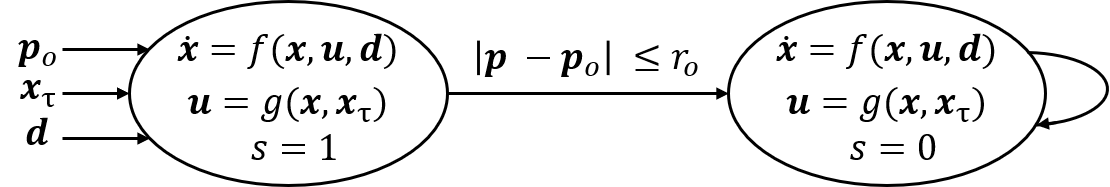
\includegraphics[width=0.4\textwidth]{figures/hybrid_system}
	\caption{Hybrid system model.}
	\label{fig:hybrid_model}
\end{figure}



\end{section}
% !TEX root = IROS2019_DNN.tex
\begin{section}{Run-time Verified Reachability for Safety} \label{sec:method}
\begin{figure*}[t]
	\centering
	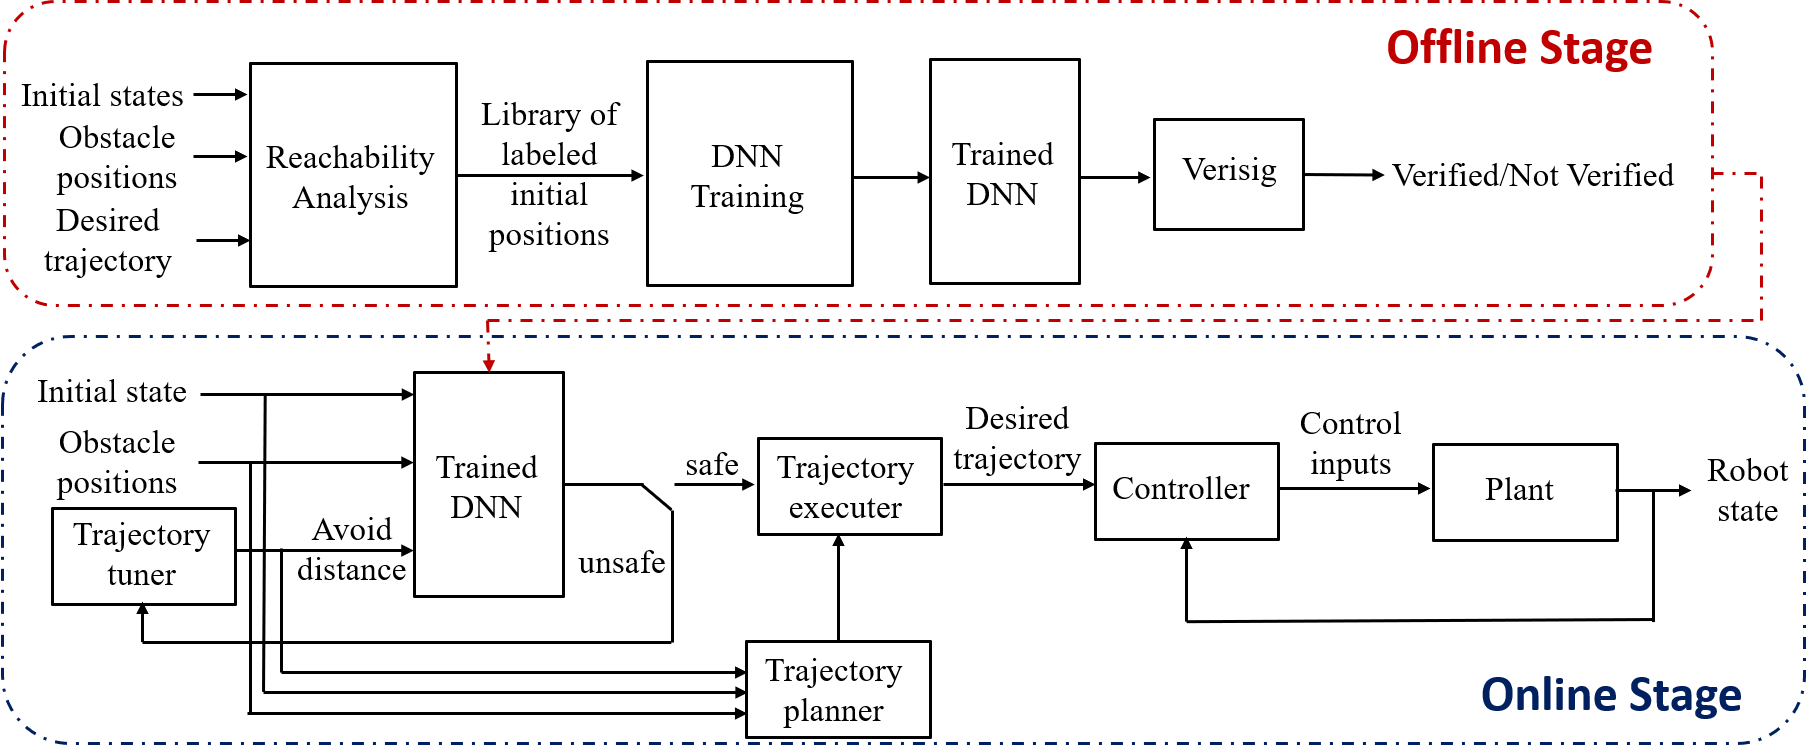
\includegraphics[width=0.8\textwidth]{figures/detailed_approach}
	\caption{Run-time verified reachability framework.}	
	\label{fig:det_app}
\end{figure*}

In this section, we describe our framework for run-time verified reachability for safety assurance of the autonomous operations. The proposed architecture is shown in Fig.~\ref{fig:det_app}.

In this work we propose a novel approach to make decisions about the safety of a trajectory at run-time using DNNs to predict the output of the reachability analysis in a very fast way. At the offline stage, obstacle free trajectories are generated from various initial positions to the given goal position. While designing the trajectory, the desired distance to keep from the obstacles (avoid distance) is specified by the user. Each initial position and avoid distance pair is labeled as safe or unsafe based on the reachability analysis. In this work, we use a simulation based reachability analysis for this particular system, however, the framework is independent from the choice of reachability tool. The aim is to predict the safety decisions of the reachability tool of choice in a fast way using DNNs. The library of labeled initial position-avoid distance pairs are used to train a DNN to predict the safety label of a different input pair. The trained DNN is then verified using Verisig and verified network is then used at online stage to make verified decisions about the safety of the trajectory from a given initial position to the goal position with a given avoid distance from the obstacles. 

The first step in our approach is the generate a trajectory library for offline training which is explained in the following section.
\subsection{Training Set Generation: Safety Labeled Initial Positions}
In order to have a network which is trained well enough to make accurate decisions, there is a need for a rich training set. In this work, the aim is to predict the safety of an initial position with a given avoid distance in a static environment. For this reason, a set of trajectories from a rich set of initial positions with different avoid distances is generated as explained in the following subsection.
\subsubsection{Trajectory Generation:}
In this work, trajectories are generated using minimum snap trajectories because of the fact that they are particularly suitable for quadrotor UAV dynamics to follow \cite{Mellinger2011}. We use an heuristic approach to avoid the obstacles in the environment, however any path planning algorithm can be used for this purpose. When there is an obstacle along the way to the goal position, a waypoint is added to the path which is away from the obstacle by the specified avoid distance ($ r_a $). Then the trajectory is generated to visit all the waypoints and the final goal position by using minimum snap trajectory generation. In Fig.~\ref{fig:trajs}, some sample trajectories with different avoid distances are shown. In Fig.~\ref{fig:traj1_025} and \ref{fig:traj1_03}, the trajectory is generated from the same initial position $ \boldsymbol{p}_0 = [0.3, 0, 1] $ with $ r_a = 0.25 $ and $ r_a = 0.3 $ respectively. In this work, it is assumed that the trajectories are generated by following the same rules.
\begin{figure}[h]
	\centering
	\subfigure[$ r_a = 0.25 $\label{fig:traj1_025}]{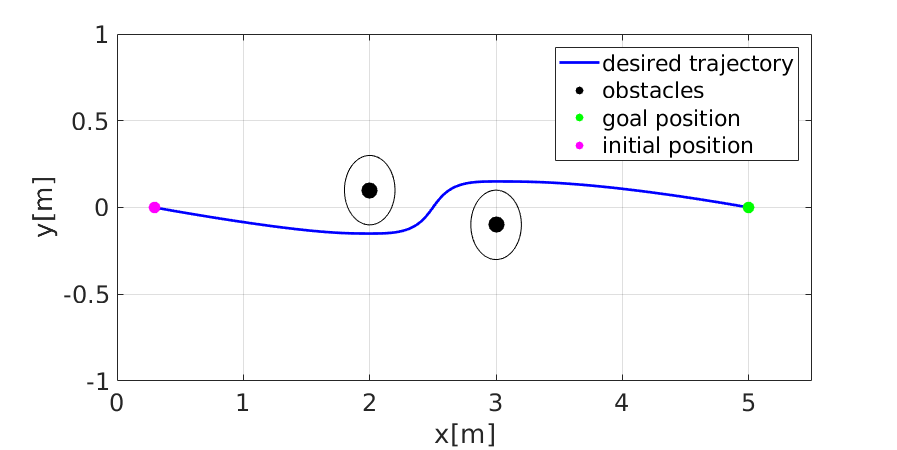
\includegraphics[width=0.22\textwidth]{figures/trajectories/traj_1}}
	\subfigure[$ r_a = 0.3 $\label{fig:traj1_03}]{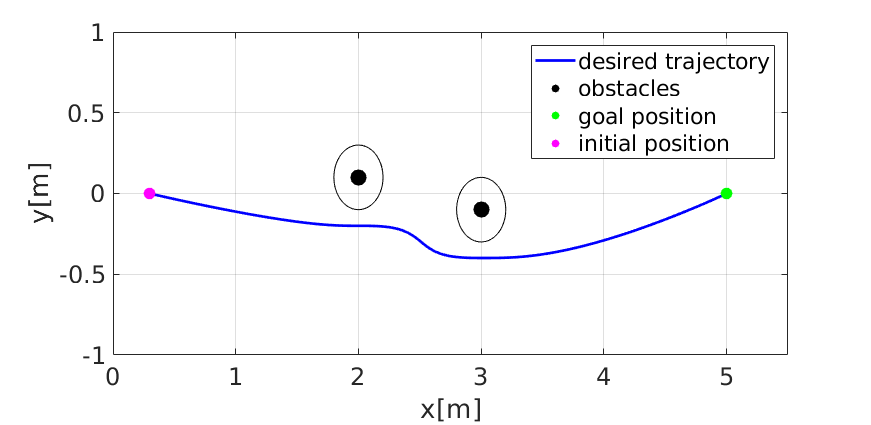
\includegraphics[width=0.22\textwidth]{figures/trajectories/traj_1_03}}
	%\subfigure[$ r_a = 0.25 $\label{fig:traj2_025}]{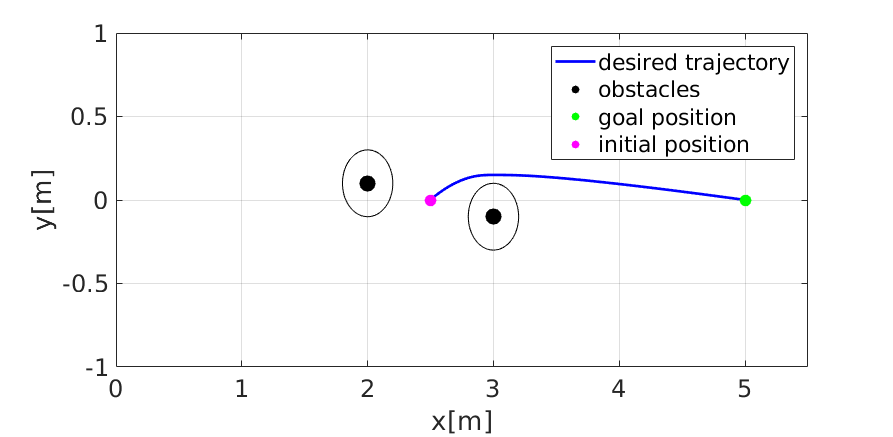
\includegraphics[width=0.22\textwidth]{figures/trajectories/traj_2}}
	%\subfigure[$ r_a = 0.3 $\label{fig:traj2_03}]{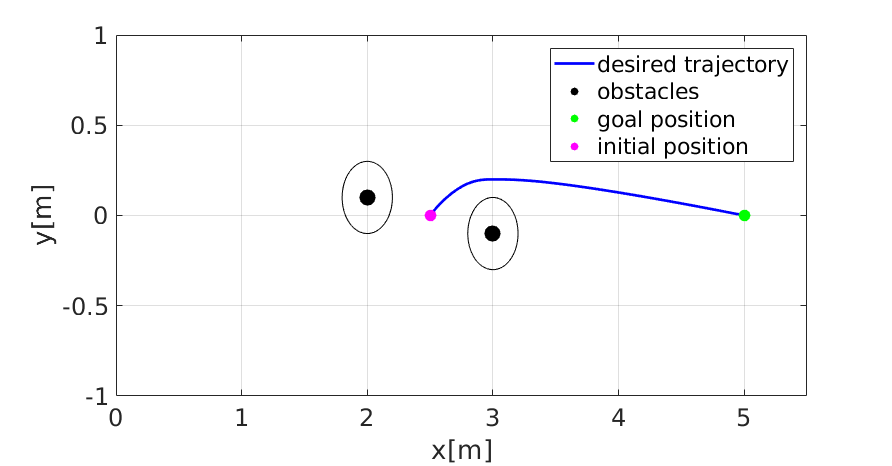
\includegraphics[width=0.22\textwidth]{figures/trajectories/traj_2_03}}
	\caption{Sample trajectories to avoid the obstacles with different avoid distances.}
	\label{fig:trajs}
\end{figure}

\subsubsection{Simulation-based Reachability Analysis:}
In order to decide if the trajectory from an initial position to the goal position is safe or not, reachability analysis needs to be performed on those trajectories. In this work, we use a simulation-based reachability analysis where the trajectories are run under the worst case scenario assumptions (i.e. worst disturbance in the environment). Under these assumptions, the maximum deviation from the trajectory at each time stamp is recorded ($ d_m(t) $). Since these maximum deviation values are recorded under worst case scenario assumptions, they can be used as upper bounds to the actual deviation from the trajectory. Then the position reachable sets are generated using as follows:
\begin{equation}
	\boldsymbol{R}(\boldsymbol{p}_\tau,t) = \{ \boldsymbol{p}(t): | \boldsymbol{p}(t) - \boldsymbol{p}_\tau(t) | \leq d_m(t) \}
	\label{eq:reach}
\end{equation}
In Fig.~\ref{fig:traj_reach}, the reachable sets generated for the trajectories in Fig.~\ref{fig:trajs} are presented.
\begin{figure}[h]
	\centering
	\subfigure[Reachable sets for the trajectory in Fig~\ref{fig:traj1_025}]{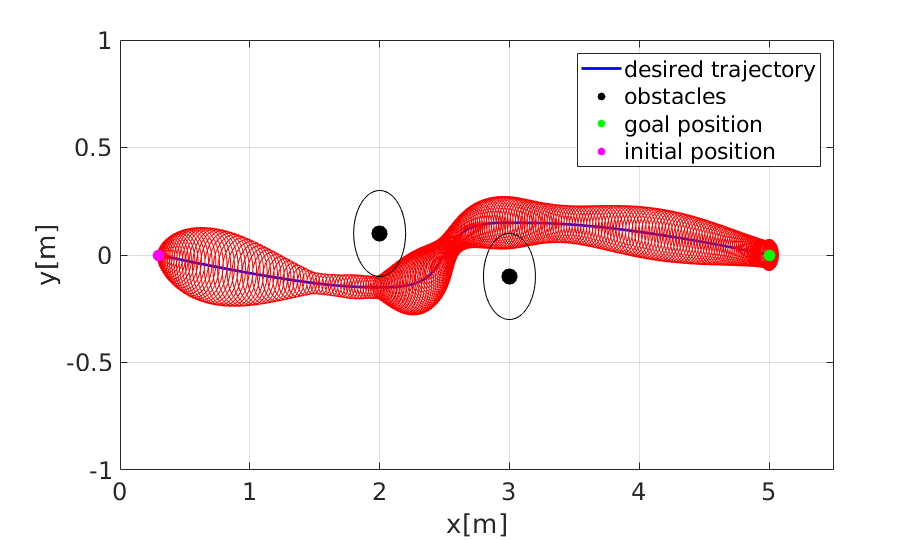
\includegraphics[width=0.22\textwidth]{figures/trajectories/traj_1_reach}}
	\subfigure[Reachable sets for the trajectory in Fig~\ref{fig:traj1_03}]{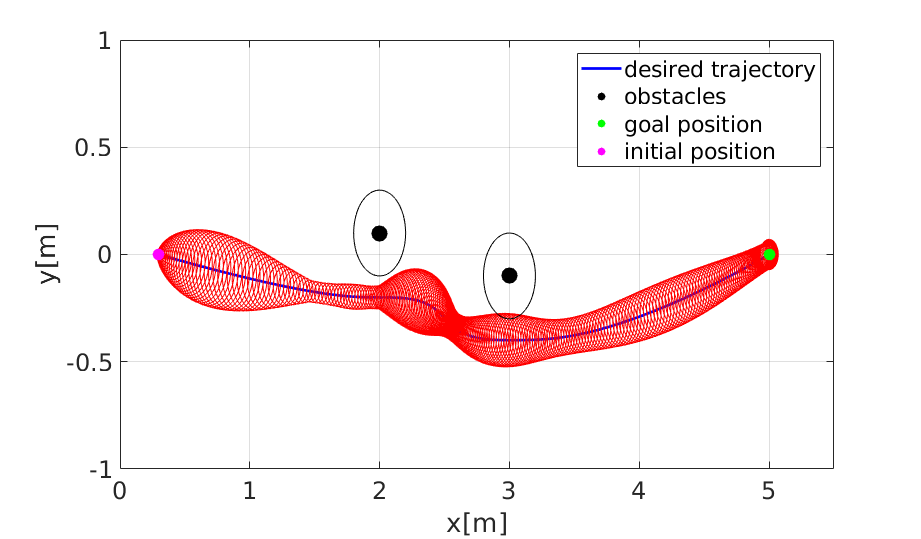
\includegraphics[width=0.22\textwidth]{figures/trajectories/traj_1_03_reach}}	
	\caption{Reachable sets for the trajectories in Fig.~\ref{fig:trajs}}
	\label{fig:traj_reach}
\end{figure}

The safety decision is made using these reachable sets. If the reachable sets of the trajectory are not intersecting with the obstacles, then the initial position and the avoid distance pair is labeled as safe:
\begin{equation}
	\begin{cases}
		s_{k,j} = 1 & \text{if   }  \boldsymbol{R}(\boldsymbol{p}_{\tau, k, j},t) \cap \boldsymbol{p}_{o,i} = \emptyset \\ 
		& \forall t \in [0,T], \forall i \in [1, \cdots, n_o], \\ 
		& k \in [1, \cdots, n_p], j \in  [1, \cdots, n_a] \\
		s_{i,j} = 0 & \text{otherwise}
 	\end{cases}
 	\label{eq:safety}
\end{equation}
where $ \boldsymbol{p}_{\tau,k,j} $ is the trajectory from $ k^{\text{th}} $ initial position with $ j^{\text{th}} $ avoid distance and $ s_{k,j} $ is the corresponding safety label. $ \boldsymbol{p}_o $ represents the $ o^\text{th} $ obstacle position, $ n_o $ is the number of obstacles in the environment, $ n_p $ is the number of initial positions in the training set and $ n_a $ is the number of different avoid distances in the training set. For instance, both trajectories in Fig.~\ref{fig:trajs} are labeled as unsafe since their reachable sets shown in Fig~\ref{fig:traj_reach} are colliding with obstacles.

In this work, we have generated a training set which includes 1886 initial positions whose $ x $ and $ y $ positions are uniformly distributed between $ [0,4.5] $m and $ [-2,2] $m respectively with $ 0.1 $m increments. During training six different avoid distances are used: $ r_a \in \{0.25, 0.3, 0.35, 0.4, 0.45, 0.5\} $. The entire training set consists of 11316 initial position-avoid distance pairs. In Fig~\ref{fig:safety_gt}, all the initial positions included in the training set are shown in the case environment. Safe initial positions are marked with green dots whereas unsafe initial positions are marked with red dots. For each avoid distance, a separate map is generated because the safety labels depend on the avoid distance as well. As can be noticed, as the avoid distance increases, number of safe initial positions also increases because the distance between the desired trajectories and obstacles becomes larger. Therefore, increasing avoid distance improves the safety, however the trajectories become longer, which is not something desirable for energy and time concerns.

\begin{figure}[H]
	\centering
	\subfigure[$ r_a = 0.25m $]{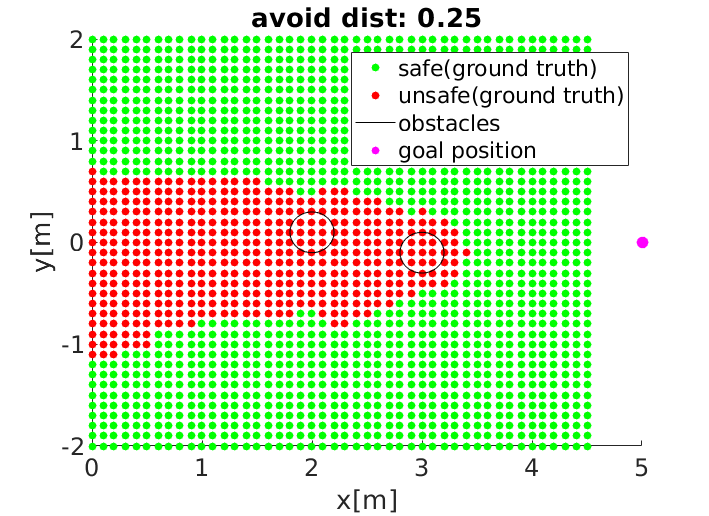
\includegraphics[width=0.15\textwidth]{figures/trajectories/training_gt_025}}
	\subfigure[$ r_a = 0.3m $]{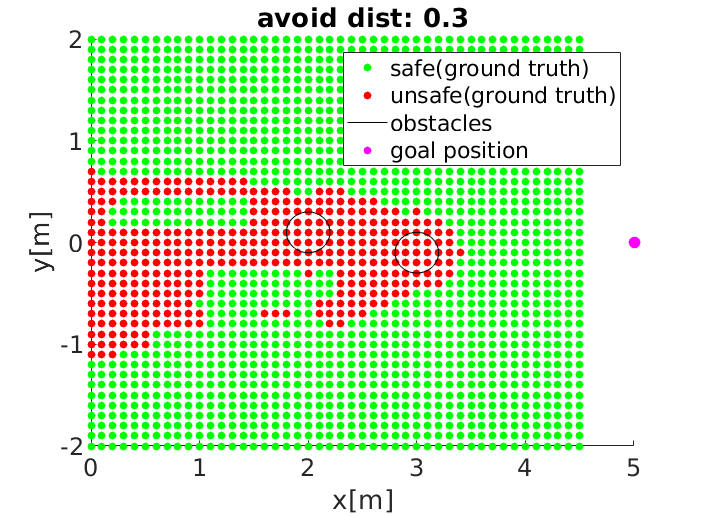
\includegraphics[width=0.15\textwidth]{figures/trajectories/training_gt_03}}
	\subfigure[$ r_a = 0.35m $]{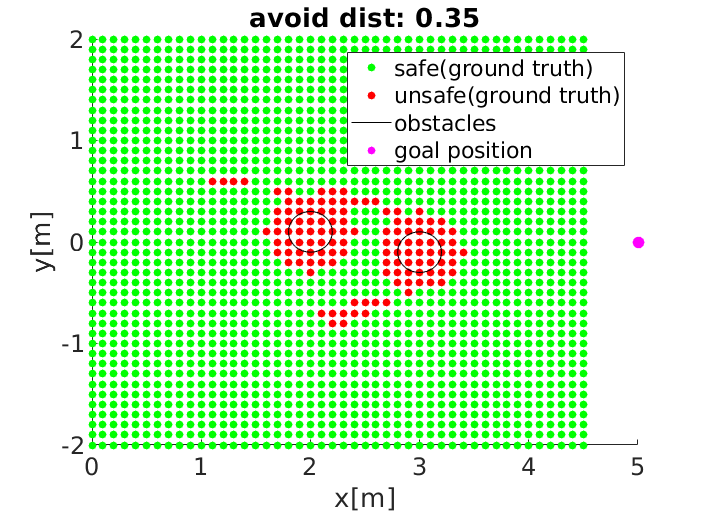
\includegraphics[width=0.15\textwidth]{figures/trajectories/training_gt_035}}
	\subfigure[$ r_a = 0.4m $]{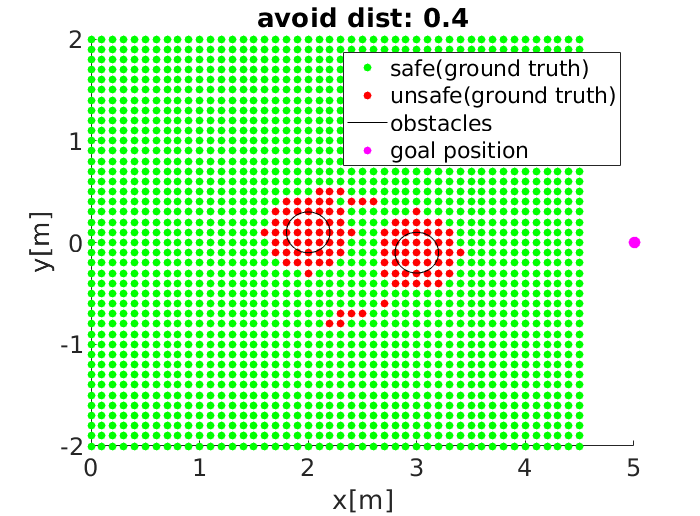
\includegraphics[width=0.15\textwidth]{figures/trajectories/training_gt_04}}
	\subfigure[$ r_a = 0.45m $]{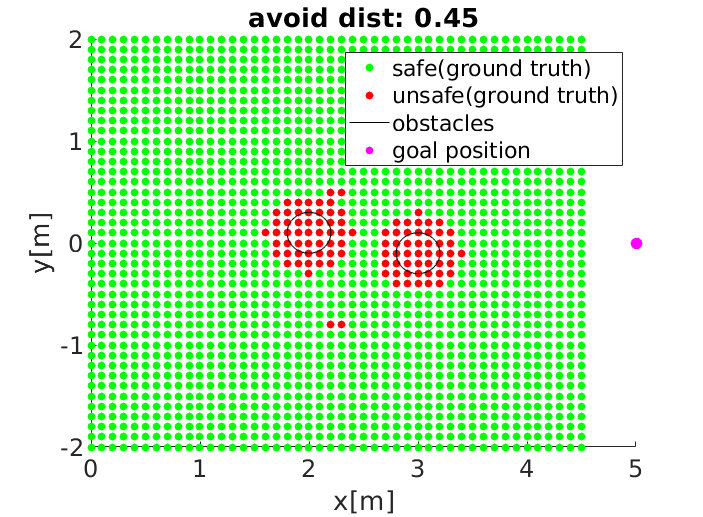
\includegraphics[width=0.15\textwidth]{figures/trajectories/training_gt_045}}
	\subfigure[$ r_a = 0.5m $]{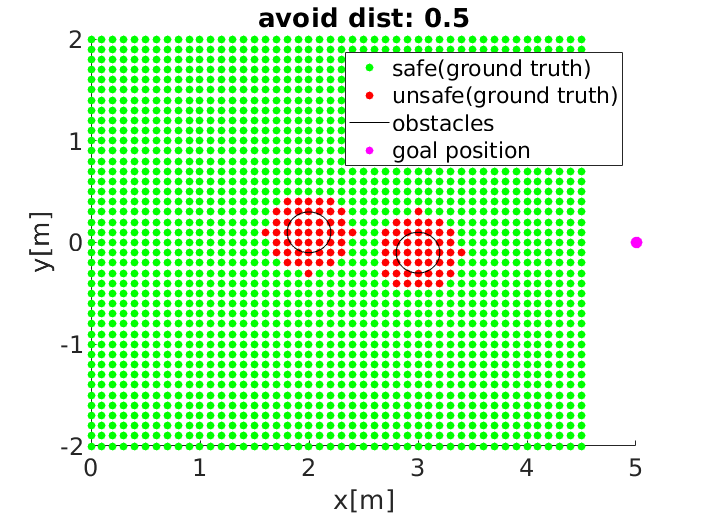
\includegraphics[width=0.15\textwidth]{figures/trajectories/training_gt_05}}
	\caption{Safety maps for the initial position in the training set with all avoid distances used in the training stage.}
	\label{fig:safety_gt}
\end{figure}

\subsection{Verified Reachability}
\subsubsection{DNN-Based Safety}
Neural networks have been used successfully in many application domains for recognizing patterns from a set of data. We are interested in classifying safe and unsafe trajectories given the initial position and the avoid distance radius.

We trained a shallow neural network (one hidden layer) with three node inputs, fifty hidden nodes, and two output nodes (one for each class).  
The network has been trained using the Neural Network Pattern Recognition Tool.
% using the standard 'trainfp' training function that has been shown to provide the best results for our training set. 
We decided to use only one hidden layer since the two classes are easy to discriminate concerning the inputs. Tests with more hidden layers (up to 50) have not shown consistent improvements. Multiple layers are in general more useful when more general features/concepts need to be classified.

Due to the high difference in the number of safe labels (~10k ) against unsafe ones (~1.2k), the training may result in returning false positive outputs (unsafe trajectory labeled safe). For this reason, we weight unsafe labels to be forty times more relevant than safe values. The training results showed 0\% False positive (FP) and around ~5\% False Negative (FN). The relatively high number of FN is more than acceptable since it is better to be over-conservative than being risky.
  
Fig.~\ref{fig:output_test} shows the output of the neural network when using the training set as input. Similarly to \ref{fig:safety_gt} each subfigure refers to a specific avoid distance radius. Dots represent the ground truth while circles the DNN output.
It is worth noting that, there are 0 FP values (red dots surrounded by green circles) while there is a certain number of FN (green dots surrounded by red circles) showing the conservative DNN behavior.
\begin{figure}[H]
	\centering
	\subfigure[$ r_a = 0.275m $]{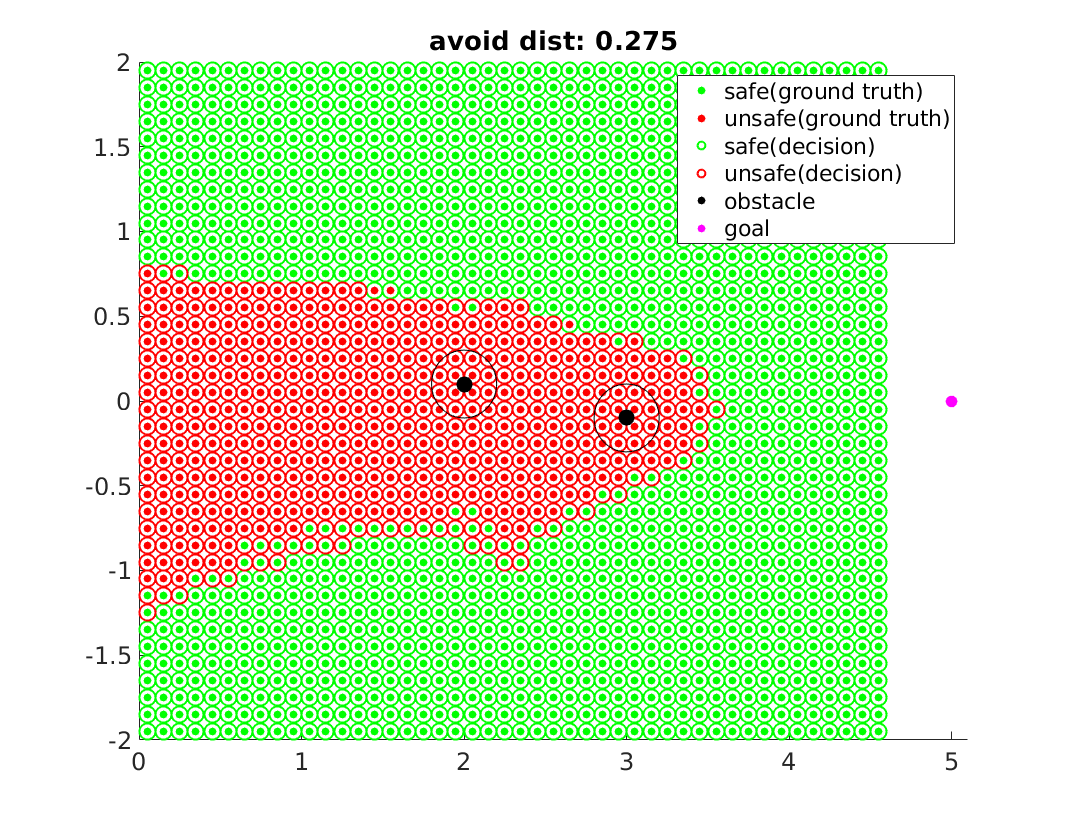
\includegraphics[width=0.15\textwidth]{figures/trajectories/testing_dec05_0275_new}}
	\subfigure[$ r_a = 0.3m $]{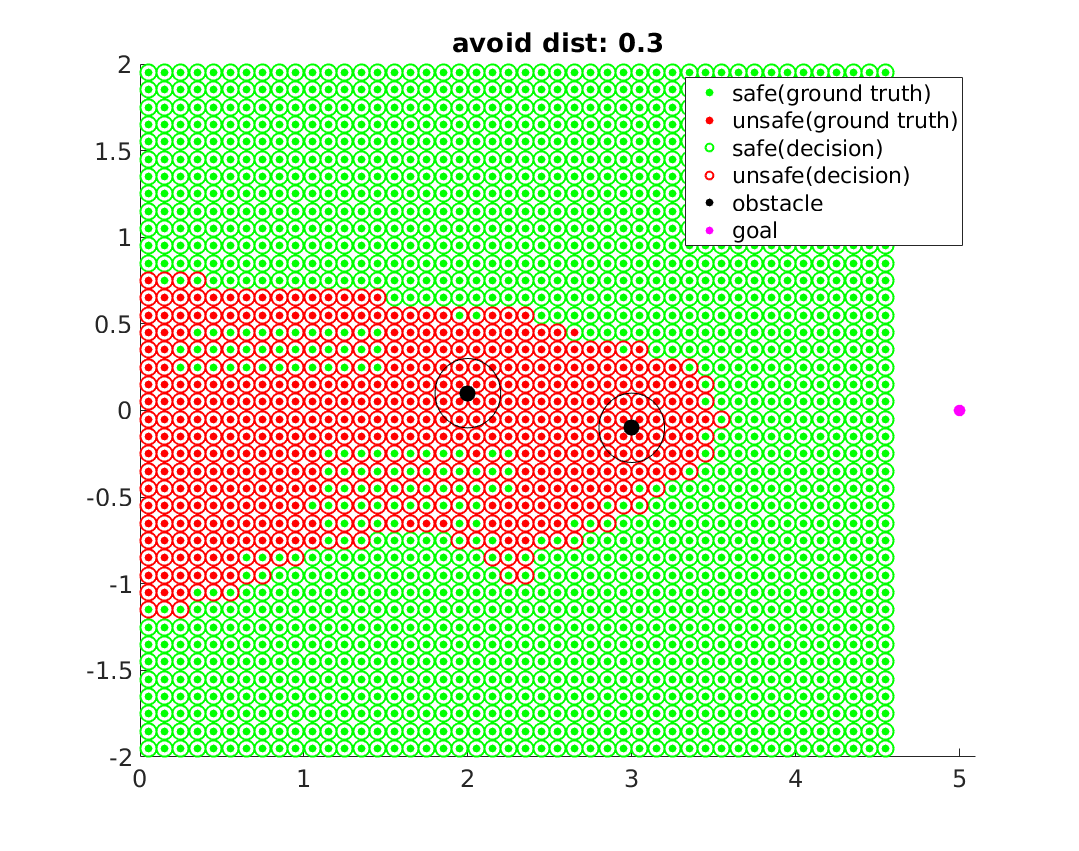
\includegraphics[width=0.15\textwidth]{figures/trajectories/testing_dec05_03_new}}
	\subfigure[$ r_a = 0.325m $]{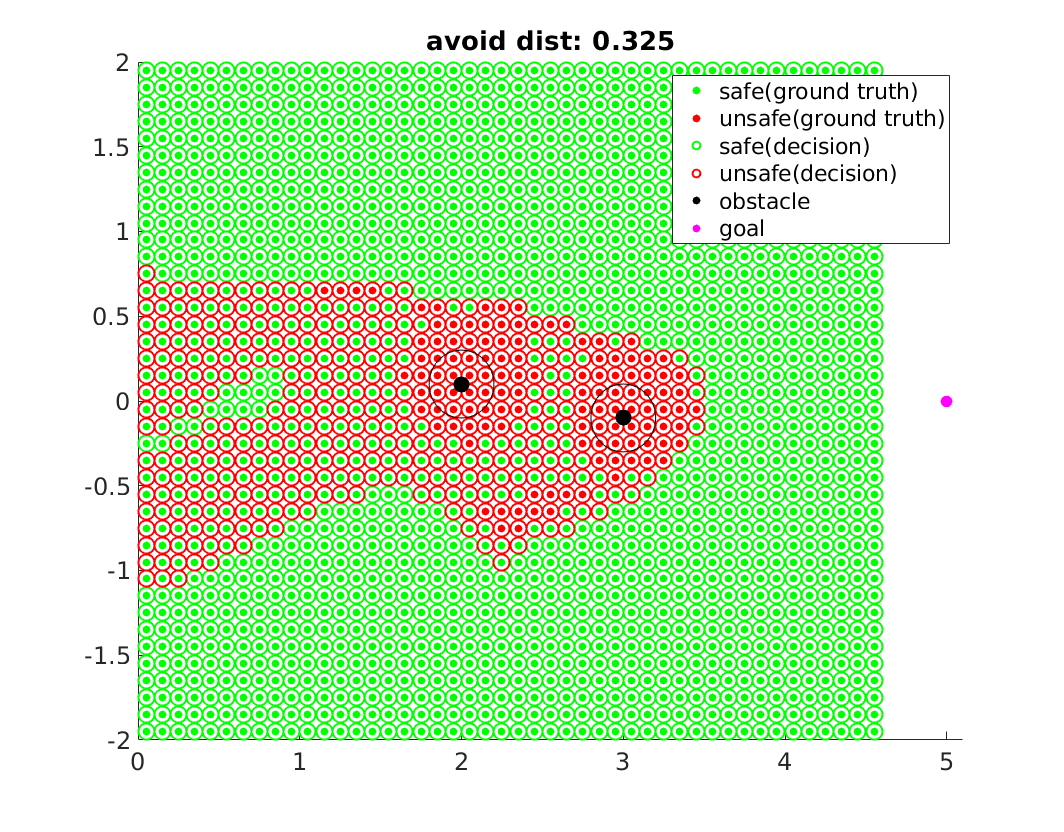
\includegraphics[width=0.15\textwidth]{figures/trajectories/testing_dec05_0325_new}}
	\subfigure[$ r_a = 0.375m $]{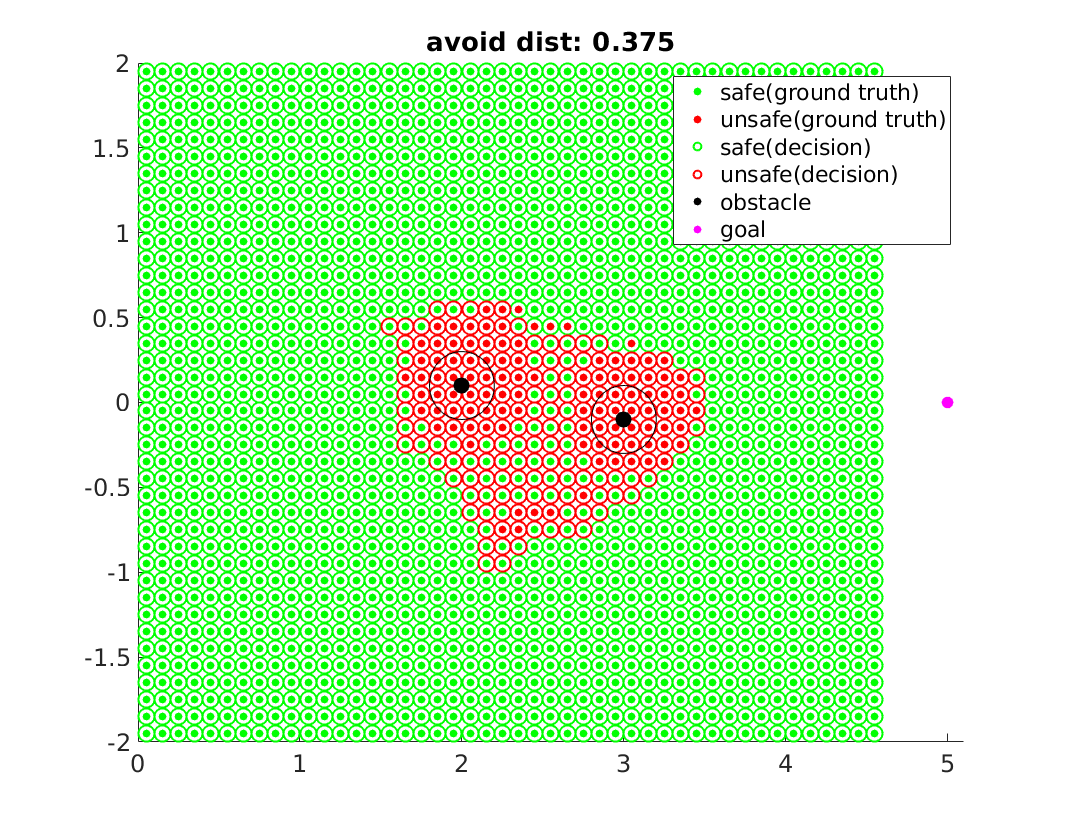
\includegraphics[width=0.15\textwidth]{figures/trajectories/testing_dec05_0375_new}}
	\subfigure[$ r_a = 0.425m $]{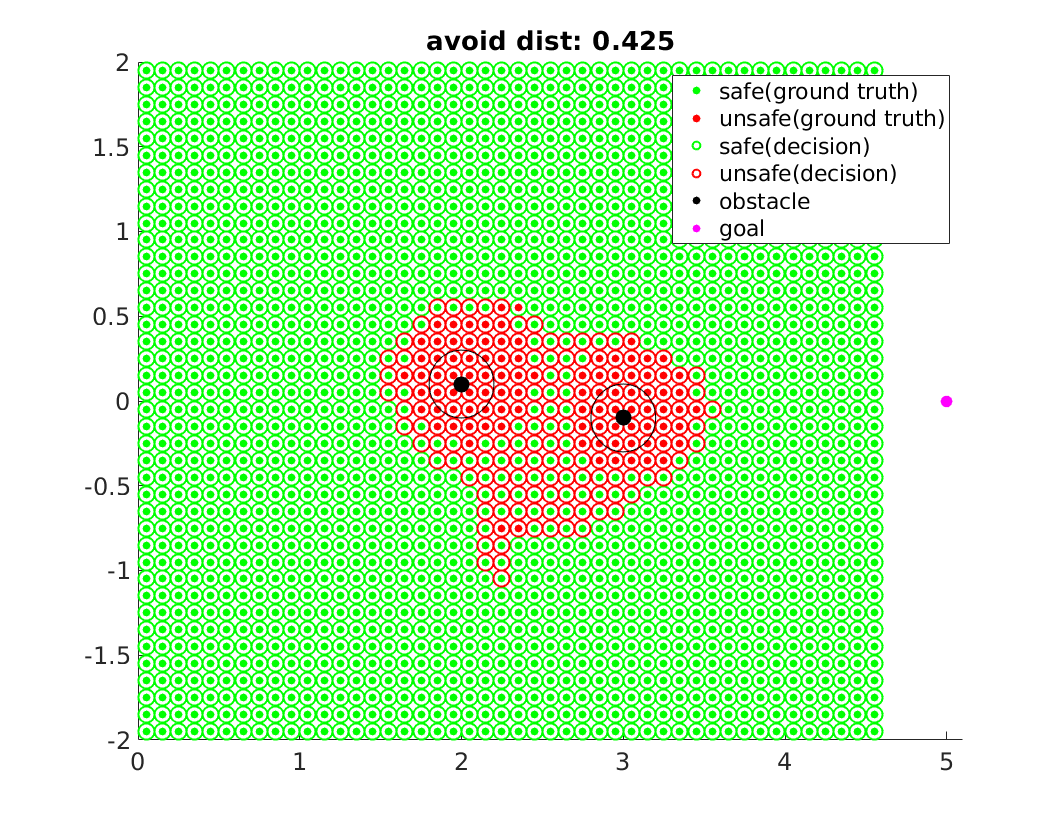
\includegraphics[width=0.15\textwidth]{figures/trajectories/testing_dec05_0425_new}}
	\subfigure[$ r_a = 0.475m $]{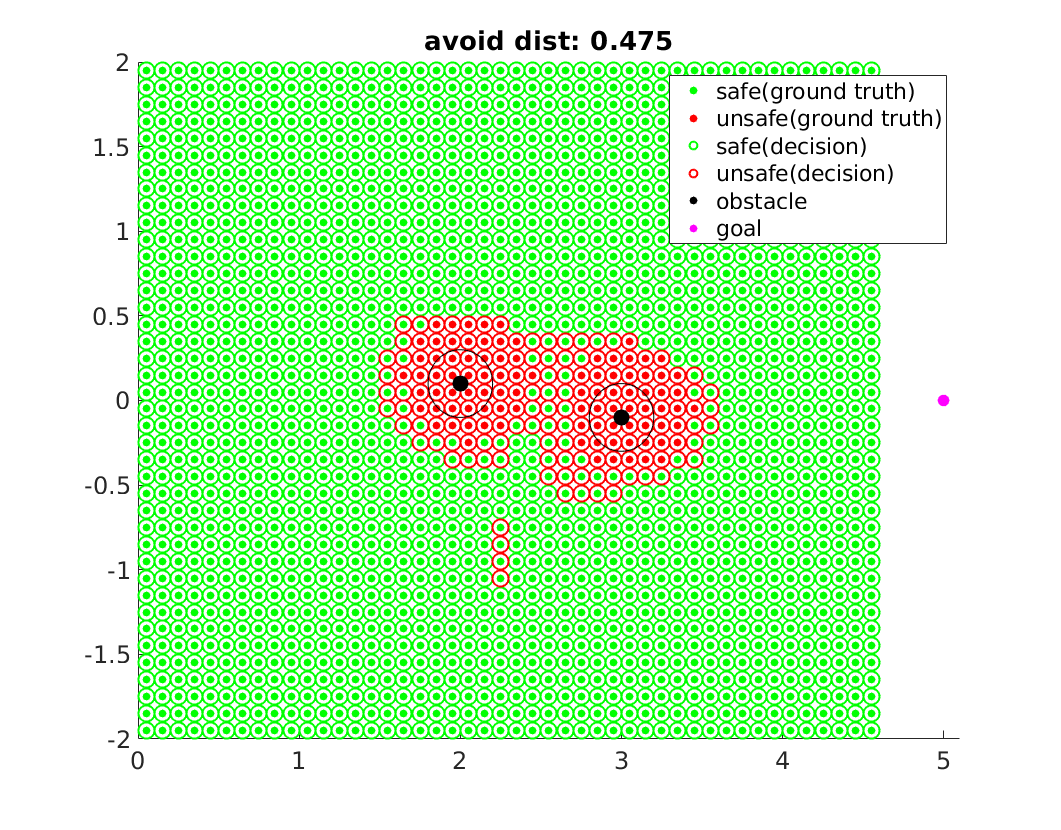
\includegraphics[width=0.15\textwidth]{figures/trajectories/testing_dec05_0475_new}}
	\label{fig:output_test}
	\caption{DNN safety decisions for test initial positions.}
\end{figure}

\subsubsection{Verisig}
Details about Verisig and how our network is verified (under what conditions) will be given here. \EY{I've left this out for now}

\end{section}
 
% !TEX root = IROS2019_DNN.tex

\begin{section}{Simulations} \label{sec:simulation}
\EY{We should discuss about what kind of simulations we're planning to show}
\end{section}
%!TEX root = IROS2019_DNN.tex

\begin{section}{Experiments} \label{sec:experiment}
\EY{We should discuss about what kind of experiments we're planning to show}
\end{section}
% !TEX root = IROS2019_DNN.tex

\begin{section}{Conclusion and Future Work} \label{sec:conclusion} 

\end{section}

%%%%%%%%%%%%%%%%%%%%%%%%%%%%%%%%%%%%%%%%%%%%%%%%%%%%%%%%%%%%%%%%%%%%%%%%%%%%%%%%

\bibliographystyle{IEEEtran}
\bstctlcite{IEEEexample:BSTcontrol}
\bibliography{references}


\end{document}

